%\documentclass{emulateapj}
%\documentclass[preprint2]{aastex}
% \documentclass[iop]{emulateapj}
\documentclass[useAMS,usenatbib]{mn2e}
\usepackage{epsfig}
\usepackage{epstopdf}
\usepackage{lscape} % Allows landscape environment to be used
\usepackage{graphicx}
\usepackage{multirow}
\usepackage{hhline}
\usepackage{amsmath}
\usepackage{gensymb}
%\usepackage{floatrow}
%\def\gtrsim{\mathrel{\hbox{\rlap{\hbox{\lower4pt\hbox{$\sim$}}}\hbox{$>$}}}}
%\renewcommand\floatpagefraction{.9}
%\renewcommand\dblfloatpagefraction{.9} % for two column documents
%\renewcommand\topfraction{.9}
%\renewcommand\dbltopfraction{.9} % for two column documents
%\renewcommand\bottomfraction{.9}
%\renewcommand\textfraction{.1}   
%\setcounter{totalnumber}{50}
%\setcounter{topnumber}{50}
%\setcounter{bottomnumber}{50}

\begin{document}

\title[Lensing Distance]{
Scintillation Distance Measurements
}

%\author{J.~D.~Emberson\altaffilmark{1,2}, Takeshi~Kobayashi\altaffilmark{1,3} \& Marcelo~A.~Alvarez\altaffilmark{1}}
%\altaffiltext{1}{Canadian Institute for Theoretical Astrophysics,
%  University of Toronto, 60 St.George St., Toronto, ON M5S 3H8, Canada} 
%\altaffiltext{2}{Department of Astronomy and Astrophysics, University
%  of Toronto, 50 St. George, Toronto, ON M5S 3H4, Canada} 
%\altaffiltext{3}{Perimeter Institute for Theoretical Physics, 31 Caroline Street North, Waterloo, ON N2L 2Y5, Canada}
%\email{emberson@astro.utoronto.ca}

%\author{Siqi Liu\altaffilmark{1,3}, Ue-Li~Pen\altaffilmark{1,2}, J-P~Macquart\altaffilmark{4}, Walter Brisken\altaffilmark{5}, Adam Deller\altaffilmark{6}}
%\altaffiltext{1}{Canadian Institute for Theoretical Astrophysics, University of Toronto, M5S 3H8 Ontario, Canada} 
%\altaffiltext{2} {Canadian Institute for Advanced Research, Program in Cosmology and Gravitation; pen@cita.utoronto.ca}
%\altaffiltext{3} {Department of Astronomy and Astrophysics, University of Toronto, M5S 3H4, Ontario, Canada; sqliu@cita.utoronto.ca}
%\altaffiltext{4} {ICRAR-Curtin University of Technology, Department of Imaging and Applied Physics, GPO Box U1978, Perth, Western Australia 6102, USA; J.Macquart@curtin.edu.au}
%\altaffiltext{5} {National Radio Astronomy Observatory, P.O. Box O, Socorro, NM 87801, USA; wbrisken@aoc.nrao.edu}
%\altaffiltext{6} {ASTRON, the Netherlands Institute for Radio Astronomy, Postbus 2, 7990 AA, Dwingeloo, The Netherlands; deller@astron.nl}
\author[Liu et al]{Siqi Liu$^{1,3}$\thanks{E-mail:\ sqliu@cita.utoronto.ca}, Ue-Li
  Pen$^{1,2}$\thanks{E-mail:\ pen@cita.utoronto.ca}, J-P Macquart$^{4}$\thanks{E-mail:J.Macquart@curtin.edu.au},
  Walter Brisken$^{5}$\thanks{Email:wbrisken@aoc.nrao.edu}, Adam Deller$^{6}$\thanks{E-mail:deller@astron.nl}\\
 $^1$ Canadian Institute for Theoretical Astrophysics, University of Toronto, M5S 3H8 Ontario, Canada \\
$^2$ Canadian Institute for Advanced Research, Program in Cosmology
and Gravitation\\
$^3$ Department of Astronomy and Astrophysics, University of Toronto, M5S 3H4, Ontario, Canada\\
$^4$ ICRAR-Curtin University of Technology, Department of Imaging and Applied Physics, GPO Box U1978, Perth, Western Australia 6102, USA \\
$^5$ National Radio Astronomy Observatory, P.O. Box O, Socorro, NM 87801, USA\\
$^6$ ASTRON, the Netherlands Institute for Radio Astronomy, Postbus 2, 7990 AA, Dwingeloo, The Netherlands\\
}

\date{\today}

\pagerange{\pageref{firstpage}--\pageref{lastpage}} 
\pubyear{2015}

\maketitle
\label{firstpage}
\begin{abstract}
We show how interstellar scintillations, combined with VLBI
measurements, can be used to measure distances.  
We apply the technique to archival data on PSR
B0834+06, concluding that for this example the plasma lenses can be
precisely modelled using the \citep{2014MNRAS.442.3338P} inclined sheet model,
resulting in two distinct lens planes.  This data strongly favours the
reconnection sheet model over turbulence as the primary source of
pulsar scattering. A global 
conformal distance degeneracy exists which allows a rescaling of the
absolute distance scale.  This degeneracy is broken if the pulsar resides in a
binary system, which is the case for most precision timing targets.
\end{abstract}
\begin{keywords}
Pulsar
\end{keywords}

\newcommand{\be}{\begin{eqnarray}}
\newcommand{\ee}{\end{eqnarray}}
\newcommand{\beq}{\begin{equation}}
\newcommand{\eeq}{\end{equation}}

\section{Introduction}

Pulsars have long provided a rich source of astrophysical information
due to their compact emission and predictable timing. One of the
weakest measurements for most pulsars is their direct geometric
distance.  For some pulsars, timing parallax or VLBI parallax has
resulted in direct distance determinations.  For most pulsars, the
distance is a major uncertainty for precision timing interpretations,
including mass, moment of inertia, and gravitational wave
direction \citep{boyle2012}.

Direct VLBI observation of PSR B0834+06 shows multiple images lensed
by the interstellar plasma.  Combining the angular positions and
scintillation delays, the authors published the derived effective
distance \citep{2010ApJ...708..232B} of approximately $1168\pm 23$ pc
for apexes whose time delays range from $0.1$ ms to $0.4$ ms, and
$1121\pm 59$ pc for $1$ ms apexes.  This represents a precise
measurement compared to all other attempts to derive distances to this
pulsar.  This effective distance is a combination of pulsar-screen and
earth-screen distances, and does not allow a separate determination of
the individual distances.  A binary pulsar system would in principle
allow a breaking of this degeneracy \citep{2014MNRAS.442.3338P}. One
potential limitation is the precision to which the lensing model can
be understood.  In this paper, we demonstrate that the lensing screen
consists of nearly parallel linear refractive structures, in two
screens.  The precise model confirms the one dimensional nature, and
thus the small number of parameters that need to be measured to
quantify the lensing screen. 

\section{Lensing}
\subsection{B0834+06}
\label{21}
Our analysis is based on the reduced apex catalog from
\citep{2010ApJ...708..232B}. Information from each identified apex includes delay $\tau$,
delay rate (differential frequency $f_D$), Right Ascension $\alpha$, declination $\delta$, error of $\alpha$ $\sigma_{\alpha}$ and error of $\delta$ $\sigma_{\delta}$. Data of each apex are collected from four dual circular polarization $8$ MHz wide sub-bands spanning the frequency range $310.5-342.5$ MHz. 

We divide the apex data into two groups according to the time delay, one group ranges from $0.1$ ms to $0.4$ ms and the other group has time delay at about $1$ ms. The statistics of the positions of the points are: for $0.4$ ms group, there are $10$ apexes in the first two sub-bands, and $14$ apexes in the last two sub-bands; for $1$ ms group, there are $5$ apexes in the first sub-band, $6$ apexes in the second sub-band, $5$ apexes in the third sub-band, and $4$ apexes in the last sub-band. 

To match the same apexes in different sub-bands, we convert the differential frequency in different sub-bands to the one in $322.5$ MHz, by $f_D/f_{\rm band}\cdot322.5$ MHz. Then we map
a total of $9$ apexes from the $0.4$ ms group, and $5$ apexes from the $1$ ms
group. This results in an estimation
for the average value in $f=322.5$ MHz and standard deviation among four sub-bands. They are listed in Table
\ref{table:apex}. The $f_D$ and $\tau$ are the arithmetic mean value of the four sub-bands $\bar{x}={\sum\limits^{n=4}_{i=1}{x_i}}/{4}$, x is for $f_D$ or $\tau$.
The mean value of $\alpha$ and $\delta$ are the weighted mean, calculated by following equation:
\begin{align*}
x=\sum\limits^{n=4}_{i=1}\frac{x_i}{{\sigma_i}^2},
\end{align*}
Here x is for $\alpha$ or $\delta$. The angle of the scintillation image away from the pulsar is defined as ${\theta}^2={\alpha}^2+{\delta}^2$. 

The method we use to calculate the error of time delay $\tau$ or differential frequency $f_D$ is by following equation:
\begin{align*}
{\sigma^2_{\rm \tau, f_D}} = \frac{\sum\limits^{n=4}_{i=1}(x_i-\bar{x})^2}{4\cdot3},
\end{align*}
and $i=4$ because there are four sub-bands. This is also how we calculate the sample error of $\alpha$ and $\delta$, marked with errorbars in Figure \ref{Doublelens}.

The way we use to calculate the population error of $\alpha$ and $\delta$, which is the $\sigma_{\alpha}$ and $\sigma_{\delta}$ listed in Table \ref{table:apex}, is related by following equation:
\begin{align*}
(\frac{1}{\sigma_{\rm \alpha, \delta}})^2 = \sum\limits^n_{i=1}{\frac{1}{{ \rm \sigma_i}^2}},
\end{align*}
where i ranges from 1 to 4, for four sub-bands, and $\rm \sigma_i$ is the error of the data in each sub-band. They are marked with circles in Figure \ref{Doublelens}.

\subsection{Solution in one lens model}
\subsubsection{Distance of the lens}
In the absence of a lens model, the
fringe rate, delay and angular position cannot be uniquely related. To interpret the data, we adopt the lensing model of
\citep{2014MNRAS.442.3338P}.  In this model, the lensing is due to projected fold caustics of a thin sheet closely aligned to the line of sight. 

How distance of the pulsar is related to the time delay $\tau$ and angle $\theta$, and how velocity is related to the differential frequency $f_D$ are related by the following equations:
\begin{align*}
\tau &=\frac{D_{\rm e}{\theta}^2}{2c}, \\
f_D  &=f\cdot\frac{\rm d\tau}{\rm dt},
\end{align*} 
where ${D_{\rm e}}$ is the effective distance. If we represent the distance of the pulsar $D_{\rm p}$, the distance of the lens $D_{\rm s}$, the effective distance is equivalent to the distance of the lens placed at the middle point of the pulsar: $D_{\rm e}={D_{\rm p} D_{\rm s}}/({D_{\rm p} - D_{\rm s}})$. 

We make a plot describing the relation of $\theta-\sqrt{\tau}$ in Figure \ref{thetatau}. A least square effective distance results in
$D_e^1=1017.1\pm 2.8$ for the  0.4\ ms apexes on lens 1 and
$D_e^2 = 1243 \pm 64$ for the 1\ ms apexes on lens 2. This indicates that the lens 1 is closer to the pulsar. 
%The error bars are large enough to allow them to be at the same distance, or perhaps a reverse distance ordering.  In this paper, we present two analyses for comparison: equidistant, and at the best fit distances. In the first case, no direct distance measurement is possible, but it nevertheless illustrates a robust interpretation of the data.

Take $D_e^1=1017.1$ pc, combined with the VLBI measured distance of the pulsar $640$ pc, the distance of lens 1 $D_{1}$, where $0.4$ ms scintillation points are refracted, is equal to $392.8$ pc. 
For $1$ ms apexes, the distance of lens 2 is equal to $422.5$ pc. Thus, the degeneracy of the distance of the screen is broken.
%From time delay $\tau$ and the angular position of the pulsar, we obtained the effective distance of the pulsar as follows: 
%for $0.4$ ms group, $D_{\rm e}=1017\pm2.8$\ pc; 
%and for $1$ ms group, $D_{\rm e}=1121\pm64$\ pc.

\subsubsection{Angular position of $0.4$ ms points}
We fit a line to the observed angular positions of the $0.4$ ms group, which has an positive angle of $\gamma=-25.2\degree$ (east of the declination axis). We use this axis to define ${\parallel}$ and define ${\bot}$ by a $90\degree$ clockwise rotation from it. 

We calculate $\theta$ from the $\theta-\sqrt{\tau}$ relation and observed $\tau$. Because all of the $\theta$ here lie on the axis defined by $\gamma$ on lens 1, so they are also denoted $\theta_{1\parallel}$ listed in the first column in Table \ref{table:apex}. Then the angular positions of the $0.4$ ms group are calculated:
\begin{align*}
{\alpha}&=-\theta \cdot {\rm sin}\gamma, \\
{\delta}&=-\theta \cdot {\rm cos}\gamma.
\end{align*}
These angular positions of the $0.4$ ms data are marked out with the scatter points on the left side in Figure \ref{Doublelens}.


\subsubsection{Angular positions of $1$ ms group}
We calculate the positions of the $1$ ms apexes in following steps. First, matching the $\theta-\sqrt{\tau}$ relation, which is plotted in Figure \ref{thetatau}, we calculate the $\theta$ from observation $\tau$. 
%Note that we define the velocity that is in the direction of the pulsar. 

Second, we consider the point with the largest $\theta$ among this $1$ ms group, represented as 5, share the same $\theta_{\parallel}$ with the point with the largest $\theta$ among the $0.4$ ms group, represented as 6. $\theta_{\bot}$ is calculated by $\theta_{\bot}=\sqrt{\theta^2-\theta_{\parallel} ^2} $. Then, by using a rotation matrix defined by $\gamma$, the position of point 5 is determined: $(-10.78,-24.35)$ mas. 

Third, to determine the position of the rest points $1-4$, we need to know the velocity of the pulsar, and then fit the $\alpha$ and $\delta$ to get the same differential frequency with the observation. To know the velocity of the pulsar, we calculated the velocity component in two directions: ${v_\parallel}$ according to the differential frequency of point $6$ in $0.4$ ms group and ${v_\bot}$.
%, the parallel direction is defined by the the axis that is $\gamma$ away from declination axis. 
$v_{\rm A5}$ (in the direction pointing from point 5 to A), which has the component in the transverse direction of the velocity can be used to calculate $v_{\bot}$, with the differential frequency $f_D$ of point $5$. The example of how the lensed image changes with the moving of the pulsar is plotted in Figure \ref{OneLensReflect}. More specifically, in a time period of $6500$ s ($\rm dt=6500$ s), we will solve two equations: 
\begin{align*}
{\rm d\tau}&=\tau(t=0{\rm s})-\tau(t=6500~{\rm s},v_{\parallel})&=f_{\rm D6}/f\cdot{\rm dt},\\
{\rm d\tau}&=\tau(t=0 {\rm s}) -\tau(t=6500~{\rm s}, v_{\rm A5}) & = f_{\rm D5} /f\cdot{\rm dt},
\end{align*}
where $f=322.5$ MHz. With the calculated $v_{\rm A5}$, we can calculate the $v_{\bot}$. Combining the $v_{\parallel}$, the total velocity of the pulsar $v_{\rm tot}$ and its angle with the north (declination) axis $\epsilon$. The result is $v_{\parallel}=180.3$ km/s and $v_{\rm A5}=159.6$ km/s. Thus the total velocity is $188.5$ km/s and $\epsilon=-8.25\degree$.

Fourth, we fit the position of the rest four points, with known proper motion of the pulsar. For example, point 4:
\begin{align*}
\tau(t=0 {\rm s}) -\tau(t=6500~{\rm s}, v_{\rm A4}) &= f_{\rm D4} /f\cdot{\rm dt},\\
v_{\rm tot}\cdot[ { \sin( {\tan}^{-1}(\alpha,\delta))\cos(\gamma)}-\cos({\tan}^{-1}(\alpha,\delta))\sin(\gamma)] &=v_{\rm A4},\\
{\alpha}^2+{\delta}^2 &= {\theta}^2
\end{align*}
We fit a line to this five calculated points, to describe these the positions of these 5 points. 
%Lying on the fitted line, point 5 share the same $\theta_{\parallel}$ as the point with the largest $\theta_{\parallel}$ in the $0.4$ ms apexes. Solving the differential frequency ${f_D}$ of this point, we can calculate the relative velocity of this point to the pulsar, called vA2, which is in the plane that is perpendicular to our line of sight with a direction pointing from point 5 to the position of the pulsar. With the same method, we obtained the $v_{\parallel}$ from the $0.4$ ms data. Thus, the total velocity of the pulsar is determined.

The time in last column of Table \ref{table:apex} is calculated with $-2{\tau}f/{f_{D}}$,
equivalent to pulsar moving at $640$ pc plane from the
original position to the lensed image position with the calculated velocity of the pulsar in that direction in one lens model.


That is one lens model fitting. Knowing time delay ${\tau}$, we can get the distance of the screen; knowing the position of point 5 and the differential frequency ${f_D}$, we can get the velocity of the pulsar; knowing the velocity and observation diffferential frequency, we can get the position of points $1-4$. %While this one lens does not fit the data, we will abandon the velocity calculated in this model.

\begin{figure}
\centering
%\epsscale{1.0}
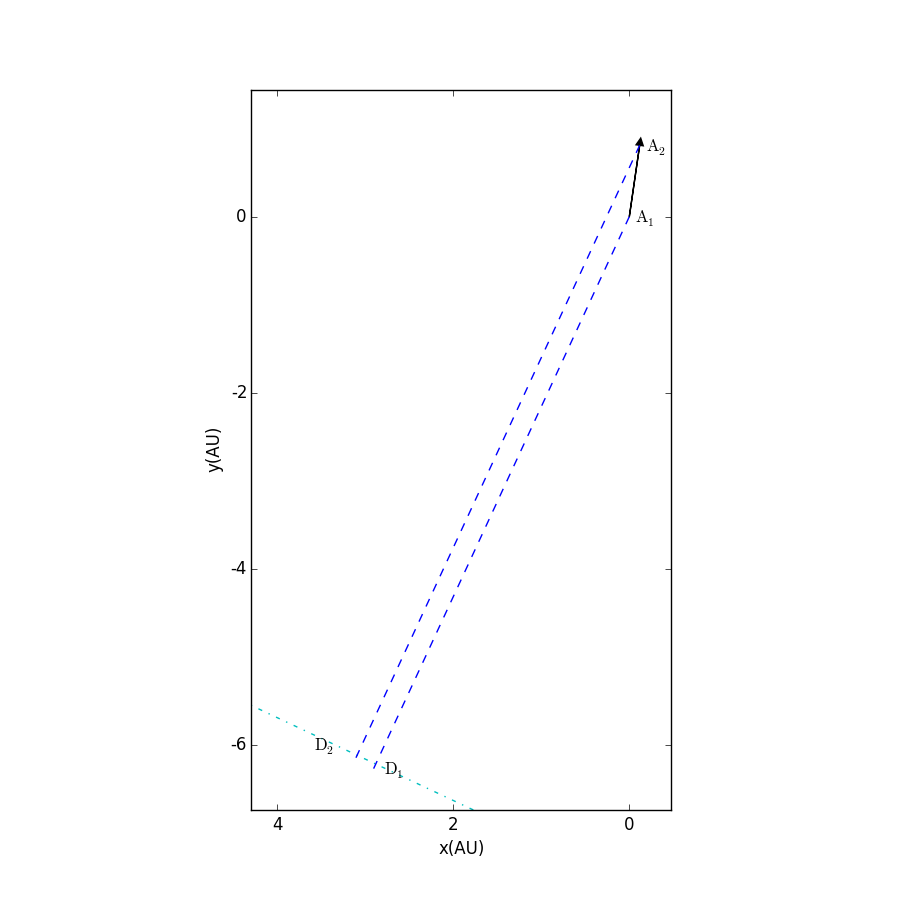
\includegraphics[width=1.0\linewidth, angle=0]{One_lens_reflection.png}
\caption{The moving of the lensed image with the moving of the pulsar. x axis and y axis are the relative distance to the position of the pulsar. $A_1$ is the original position of the pulsar, and $A_2$ is the position of the pulsar after 650000s (7.5 days). Dash line is the line of the incoming light. Dot dash line is the place where lensed image on lens 1 lies. $D_2$ is the place where the lensed image lie when the pulsar moved to $A_2$.}
\label{OneLensReflect}
\end{figure}

%\begin{figure}
%\centering
%\epsscale{1.0}
%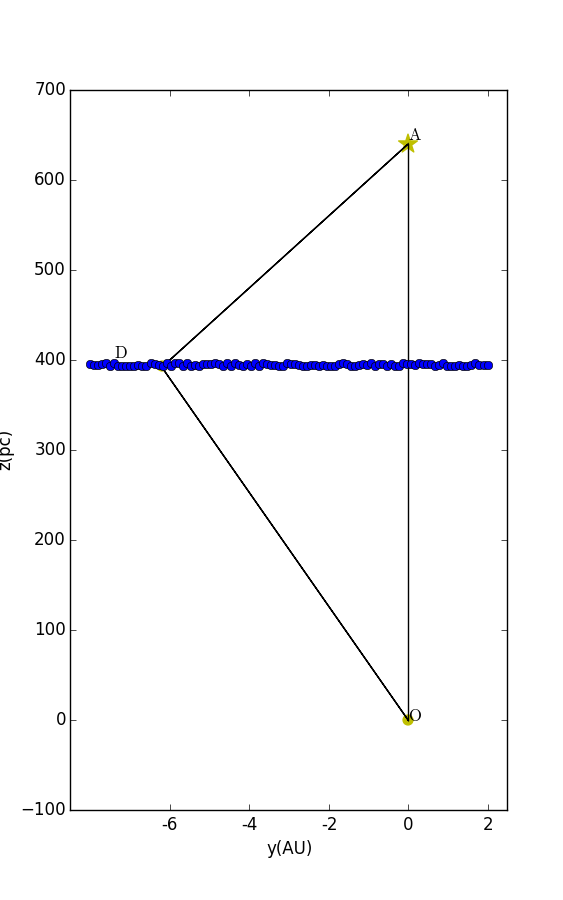
\includegraphics[width=1.0\linewidth, angle=0]{One_lens_light_path.png}
%\caption{This shows the light path of lensed/ unlensed image. The solid line on the right is the light directly emits from the pulsar to the observer. The two solid lines on the left are the lensed path. The curved line in the middle is the where lens 1 lie. X axis represents the distance in declination direction, and y axis represents the radial distance.}
%\label{OneLensLightPath}
%\end{figure}


\subsection{Discussion of one lens model}

The $0.4$ ms group lens solution appears consistent with the premise of the inclined
sheet lensing model \citep{2014MNRAS.442.3338P}.

For $1$ ms group, lens 2
only images a subset of the lens 1 images.  This could happen if
lens 1 screen is just under the critical inclination
angle, such that only $3-\sigma$ waves lead to a fold caustic.  If the lens 2 was at a critical angle, the chance of encountering a
somewhat less inclined system is of order unity.
%For the $0.4$ ms apexes, the one lens model could perfectly interpret the observation. 
More surprising is the absence of a single refraction
image of the pulsar, which is expected at position J.  This could
happen if the maximum refraction angle is just below critical, such
that only rays on the appropriately aligned double refraction can form
images.  This scenario predicts that at frequencies just below $300$
MHz, or a few weeks earlier in time, the pulsar should be seen at
position J. We made a plot of the refraction angle $\beta$ in the
direction that is transverse to the first lens plane in Figure
\ref{vtrans}.  From our calculation, it takes $22$ days for the puslar
to move from point 1 on lens 1 to J, and it takes $44$ days
for the pulsar to move from point 5 on lens 1 to J.  The data
spans about 10\% in frequency, making it unlikely that single lens
image J would not be seen due to the larger required refraction
angle.  Instead, we speculate that the fold caustic could have formed
near double lens image 1, and thus only intersections with the closer
lens plane caustic south of image 1 are double lensed.

\subsection{Double lens model}
\label{doublelensmodel}
\subsubsection{Solving the double lens model}
%The $v_{\parallel}$ to the plane should be equal. While for the calculated positions of $1$ ms apexes, they do not. 
We denote the position of the pulsar point A, position of the lensed image on lens 2 point H, position of the lensed image on lens 1 point B, position of the observer point O, pedal from the pulsar to line HJ point J, the pedal from point H to line BD point F, and the pedal from point B to line HJ point G, for easier discussion.
%As what Figure \ref{first_reflect} shows, AH should be perpendicular to HE, lens 2. 
%The plane where the light was refracted should be transverse to the line that connects the pulsar and the lensed image. 
Because points $1-4$ share the approximately same time delay with point $5$, the lens where the image formed should be at the same distance away from us. The only reasonable position of screen (line HJ) that fits all these five points, marked with a solid line in Figure \ref{Doublelens}.  
%However, in this senario, the screens cross each other, which means HE crosses with each other. 
That is unrealistic for the structure of the interstellar medium. 
%Thus, on the plane which is perpendicular to our line of sight, the incoming line should be in agree with the refraction line.
% If the light of the pulsar are being refracted by one interstellar medium lens, they should be distributed along a line like the axis of the $0.4$\ ms group, and we already know that all $1$ ms lensed images lie on the solid line in Figure \ref{Doublelens}, the only possible position will be J, which is the pedal of the position of the pulsar to the screen. 

Therefore, we consider another model candidate: the double lens model. Respective calculation shows that the light is first refracted by the lens 2 and then refracted by lens 1. 

The first step is to calculate the position of J. We make an estimate of the distance of J by the $1$ ms $\theta-\tau$ relation, and then we calculated the position of J by matching the time delay of point 2 and point 5. The result shows that lens 2 is $425$ pc away from us. And its position is marked in Figure \ref{Doublelens}. Because J is the pedal to lens 2, we made a line that is perpendicular to AJ, the solid line in Figure \ref{Doublelens}. This is lens 2.
%calculate the position of the far lens (lens $1$) and the near lens (lens $2$). As what has been discussed previously, the solid line is considered to be the far lens, where the positions have a larger effective distance. And the near lens is considered to be the lines that is perpendicular to the $0.4$ ms group axis. 

The second step is to find the matched pairs of those two lenses. By try and error, we found that the 5 points in $0.4$ ms group that have the largest $\theta$ should be the candidates where lens 1 lie.  These five matched lines are marked with dot dash lines in Figure \ref{Doublelens} and their values are listed in the first two columns in Table \ref{table:double_lens_compare}. They are the located at a distance $392.8$ pc away from us. Here we define three distances:
\begin{align*}
D_{p2}&=640~{\rm pc}-425.0~{\rm pc} =215.0~{\rm pc},\\
D_{12}&=425~{\rm pc}-392.8~{\rm pc} =32.2~{\rm pc},\\
D_{1}&=392.8~{\rm pc}- 0~{\rm pc} = 392.8~{\rm pc}, 
\end{align*} 
where $D_{p2}$ is the distance from the pulsar to lens 2, $D_{12}$ is the distance from lens 2 to lens 1, and $D_{10}$ is the distance from lens 1 to the observer.
%We calculated with the distance of the screen which is calculated in the one lens model, and then move the distance of the far screen little by little to make the calculated time delay match the observation resul

Figure \ref{first_reflect} and Figure \ref{second_reflect} are examples of how light are being refracted on the first lens plane and the second lens plane. We specifically chose the point with $\theta_{1\parallel}$ equal to $-17.44$ mas on lens $1$ for instance. We solve the solutions in double lens model by following equations:
\begin{align*}
\frac{\rm JH}{D_{p2}}&=\frac{\rm HG}{D_{12}},\\
\frac{\rm FB}{D_{12}}&=\frac{\rm BD}{D_{1}}.
\end{align*}

The solved positions are plotted in Figure \ref{Doublelens}, and respective time delays and differential frequencies are listed in Table \ref{table:double_lens_compare}. For the error of time delay $\tau$, we just use the following equation: 
\begin{align*}
(\frac{\sigma_{\rm tot}}{\tau_2})^2 = (\frac{\sigma_{\tau1}}{\tau_1})^2+(\frac{\sigma_{\tau2}}{\tau_2})^2,
%\frac{\sigma_{\rm tot}}{\tau_2} = (\frac{\sigma_{\rm 1sample}}{\tau_1})^2+(\frac{\sigma_{\rm 2sample}}{\tau_2})^2,
\end{align*}
where $\sigma_{\tau1}$ represents the sample error from the $0.4$ ms group on lens $1$, and $\sigma_{\tau2}$ represents the sample error from respective $1$ ms group on lens 2, $\tau_1$ is the time delay from $0.4$ ms group, and $\tau_2$ is the time delay from respective $1$ ms group.

\subsubsection{Comparing calculated result in double lens model and observation data}
Comparing $\tau$, we time delay for these five points, and list the results in Table \ref{table:double_lens_compare}. For point 2 and 5, they fit perfectly because these are the two points that we use these to calculate the position of J; for the rest three points, all of the calculated results are still within $3-\sigma$ region of the observation time delays.

To compare differential frequency $f_D$, we need to calculate the velocity of the pulsar and the velocity of the lens. We consider lens 1 to be relative static, both the velocity of the pulsar and the velocity of lens 2 mentioned later are the relative velocities to lens 1.
%the veloicity calculated here are the velocity of the pulsar that is relative to the lens 1, and we consider the velocity of lens 2 is also the relative value to lens 1. 
To calculate the velocity of the pulsar, we need two components, the $v_{\parallel}$ in $\theta_{\parallel}$ direction, and $v_{\bot}$ in $\theta_{\bot}$ direction. For $v_{\parallel}$, we still use the velocity that is calculated in $0.4$ ms group in one lens model, that is $180.3$ km/s. For the velocity of lens 2, because it is a line, and we do not consider radial velocity, so it could only be in the direction of AJ. However, by calculation, the $\angle$DAH is $98\degree$ by calculation, that means $v_{\bot}$ and $v_{\rm lens2}$ are nearly degenerate. In the following discussion, we consider lens 2 to be static and only take $v_{\bot}$ into account.

To calculate $v_{\bot}$, we choose the point 2, which has the smallest errorbar of differential frequency. In a time period of $6500$ s, we solved that the $v_{\bot}$ should be $7.3$ km/s, in the direction pointing from B to D, to make the calculated $f_{D2}$ match the observation $f_D$. Thus the $v_{\rm tot}$ is solved to be $192.6$ km/s, with an angle $\epsilon=4.59\degree$ west of north, which is marked on the top of the star in Figure \ref{Doublelens}.

With this velocity of the pulsar, we calculate the differential frequency of point 1,3,4 and 5. Results are listed in Table \ref{table:double_lens_compare}. The calculated results all lie in the $3-\sigma$ region of the observation data. 

%table one for 1ms positions

\begin{table*}
\centering
%\label{apex1ms}
%\resizebox{!}{1cm}{
\begin{tabular}{llllllllll}
\hline
$\theta_{1\parallel}$(mas) &$f_D$(mHz) & $\sigma_{f_D}$(mHz) & $\tau_1$(ms) & $\sigma_{\tau1}$(ms) & $\alpha$(mas) & $\sigma_{\alpha}$(mas) & $\delta$(mas) & $\sigma_{\delta}$(mas) & $t_i$(day)\\
\hline
 -8.29   & -12.94                            & 0.19      & 0.0845  & 0.0005          & 2.87    & 0.11                                     & -8.201     & 0.088      & -49.9                                \\

-10.71   &-16.80                             & 0.28      & 0.14123 & 0.0009         & 3.86    & 0.07                                     & -10.563    & 0.053      &-64.5                                \\

-12.36   &-18.92                            & 0.23      & 0.188   & 0.002           & 5.06    & 0.20                                      & -10.58    & 0.13      &-74.4                        \\

-13.44 & -20.40                             & 0.49      & 0.222   & 0.003           & 5.55    & 0.30                                      & -11.73    & 0.21      &-80.8                                \\

-13.86 &-21.17                            & 0.61      & 0.236   & 0.002           & 5.12    & 0.43                                     & -12.56    & 0.31      &-83.4                                \\

-14.63   &-22.32                            & 0.47      & 0.2633  & 0.0003          & 6.16    & 0.14                                     & -14.15    & 0.10       &-88.0                                \\

-16.29   &-24.63                            & 0.40       & 0.327  & 0.003          & 6.49    & 0.29                                     & -14.06    & 0.20       &-98.0                                \\

-16.57  &-24.94                            & 0.44      & 0.338 & 0.0003         & 8.29    & 0.42                                     & -14.37    & 0.32      &-99.7                                \\

-17.44   &-26.09                            & 0.36      & 0.3743 & 0.0006         & 8.53    & 0.52                                     & -15.74    & 0.42      &-105                               
\\ \hline
$\cdots$&         -35.06                           & 0.52                               & 0.9495               & 0.0016                              & -15.23  & 0.69                                     & -21.06   & 0.70   &-202                                   \\

$\cdots$ & -38.31                           & 0.64                               & 0.97633              & 0.00088                             & -15.02  & 0.48                                    & -20.74   & 0.38  &-190                                    \\
$\cdots$ & -40.17                           & 0.55                               & 1.0045              & 0.0079                             & -14.14  & 0.66                                    & -22.27   & 0.62  &-187                                   \\

$\cdots$ & -41.27                           & 0.54                               & 1.0370              & 0.0032                              & -11.28  & 0.93                                     & -19.2   & 1.1   &-188                                   \\

$ \cdots$ & -43.08                           & 0.44                               & 1.0663              & 0.0050                              & -8.4   & 1.7                                      & -24.1   & 1.4   &-185   \\
 \hline                                 
\end{tabular}
\caption{ $0.4$ ms and $1$ ms observation data and calculated data. 
The upper part of the table list the $0.4$ ms group data, while the $1$ ms group lie in the lower part of the table. 
Observation data include the differential frequency $f_D$, time delay $\tau$ from scintillation measurement ($\tau_1$ for $1$ ms data and $\tau_2$ for $0.4$ ms data); $\alpha$ and $\delta$ from the VLBI measurement. The method of how to calculate the error of time delay, differential frequency and the last column time is mentioned in Section \ref{21}.}
% $\theta_{1\parallel}$, the angle of the $0.4$ ms group with the component in the axis defined by $\gamma$, are derived from the $\theta-\tau$ relation plotted in Figure \ref{thetata}
\label{table:apex}
\end{table*}

\begin{table*}
\centering
\resizebox{\linewidth}{!}{
\begin{tabular}{llllllll}
\hline
$\theta_{1\parallel}$ (mas)  & $\tau_2$(ms) & $\sigma_{\rm tot}$(ms)  & $\tau_C$(ms) & $f_D$(mHz)  &$\sigma_{f_D}$(mHz)      &  $f_{DC}$(mHz)& $t_j$(day) \\ \hline
-13.86  &    0.9495     &0.0095    & 0.955       & -35.1     &1.3 & -37.22 & -22\\ 
-14.63  &   0.9763    &0.0015   & 0.9763*       & -38.3 &1.0   & -38.31$\dagger$ & 0\\ 
-16.29  &   1.005    &0.011   & 1.0272      & -40.17 &0.86    & -40.64 & 0\\ 
-16.57  &    1.0370     &0.0033    & 1.036        & -41.27 &0.90   & -41.04 & 0\\ 
-17.44  &  1.0663     &0.0052    & 1.066*        & -43.08 &0.74  &-42.26 & -44\\ \hline
\end{tabular}
}
\caption{Comparison of time delay $\tau$ and the differential frequency $f_D$ of the observation data and the calculated result in double lens model. $\theta_{1\parallel}$ is the angle of the $0.4$ ms group with the component in the axis defined by $\gamma$. $\theta_{2\parallel}$ is the angle of the $1$ ms group with the component in the axis defined by $\gamma$. The values with star symbols on them are the points that we use to calculate the position of J and the point with a $\dagger$ symbol is the point that we use to calculate the velocity of the pulsar $v_{\rm A2}$.}
\label{table:double_lens_compare}
\end{table*}
%\end{table}


%\begin{figure*}
%\centering
%\epsscale{1.0}
%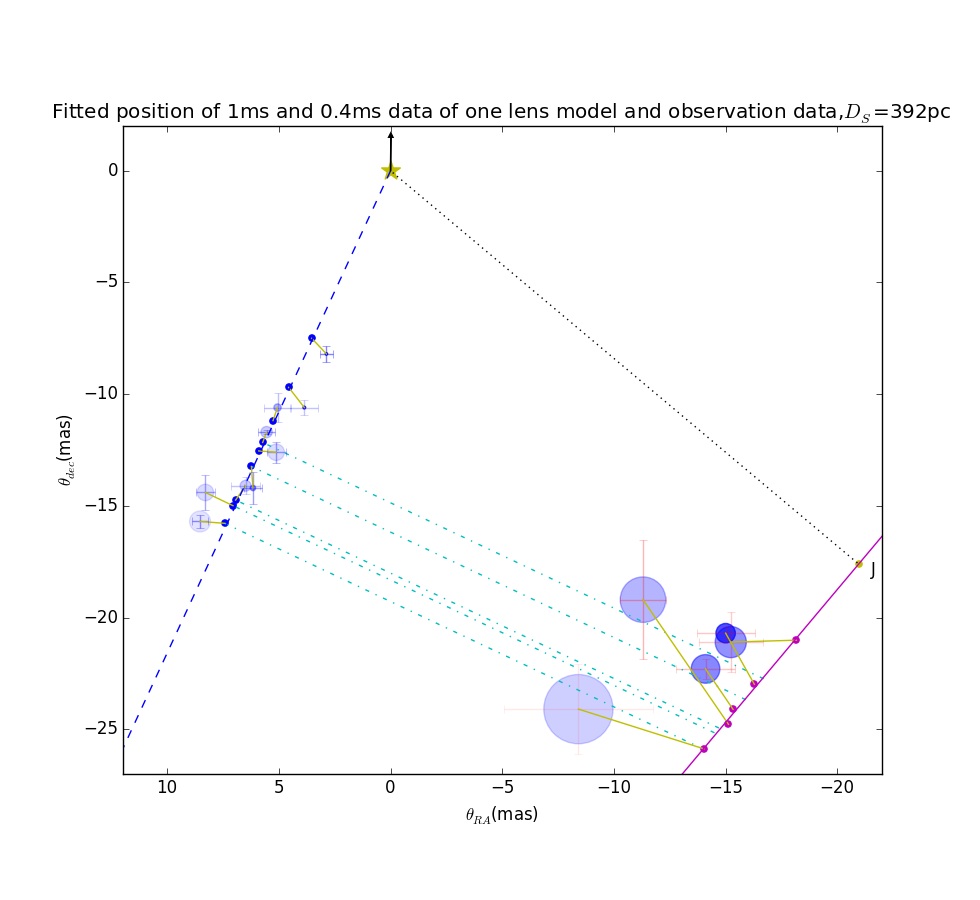
\includegraphics[width=0.8\textwidth, angle=0]{One_lens_640_392_392.png}
%\includegraphics{zN.eps}
%\caption{Fitted position of $1$ms and $0.4$ms data of one lens model and observation data. In both apexes regions, the position of the screen locate at $392.82$pc. Blue points on the left side are the points that fitted from the $f_D$ and $\tau$ of from the $0.4$ms observation. Blue line is the fitted line of $0.4$ms apex positions, with a $25.2$ degree west of the north. The points lie on the left side with errorbars, are the observation points together with their sample errors; while the transparent circles are plotted with population errors, where smaller transparent data are darker. Short solid lines between them are the matched positions of the apexes in $1ms$ region and $0.4ms$ region, which share the same $\theta_{\parallel}$. The points on the right side are the points that fitted from the $f_D$ and $\tau$ of the $1$ms observation with an avearage of four bandwidths. Solid line is the fitted line of these positions. Those points with errorbars nearby are the observation points together with their sample errors, while the transparent circles are plotted with population errors. The dotted line on the top right side is vertical to the solid line. Short solid lines connect the observation points and the fitted positions. Middle lines connect the $0.4$ms and $1$ms fitted positions with the same $\theta_{\parallel}$. The velocity of the pulsar is $199981$m/s, with a degree $0.0007$ radian east of north, which is marked out at the top of the figure.  }
%\label{Onelens_392}
%\end{figure*}

%\begin{figure*}
%\centering
%\epsscale{1.0}
%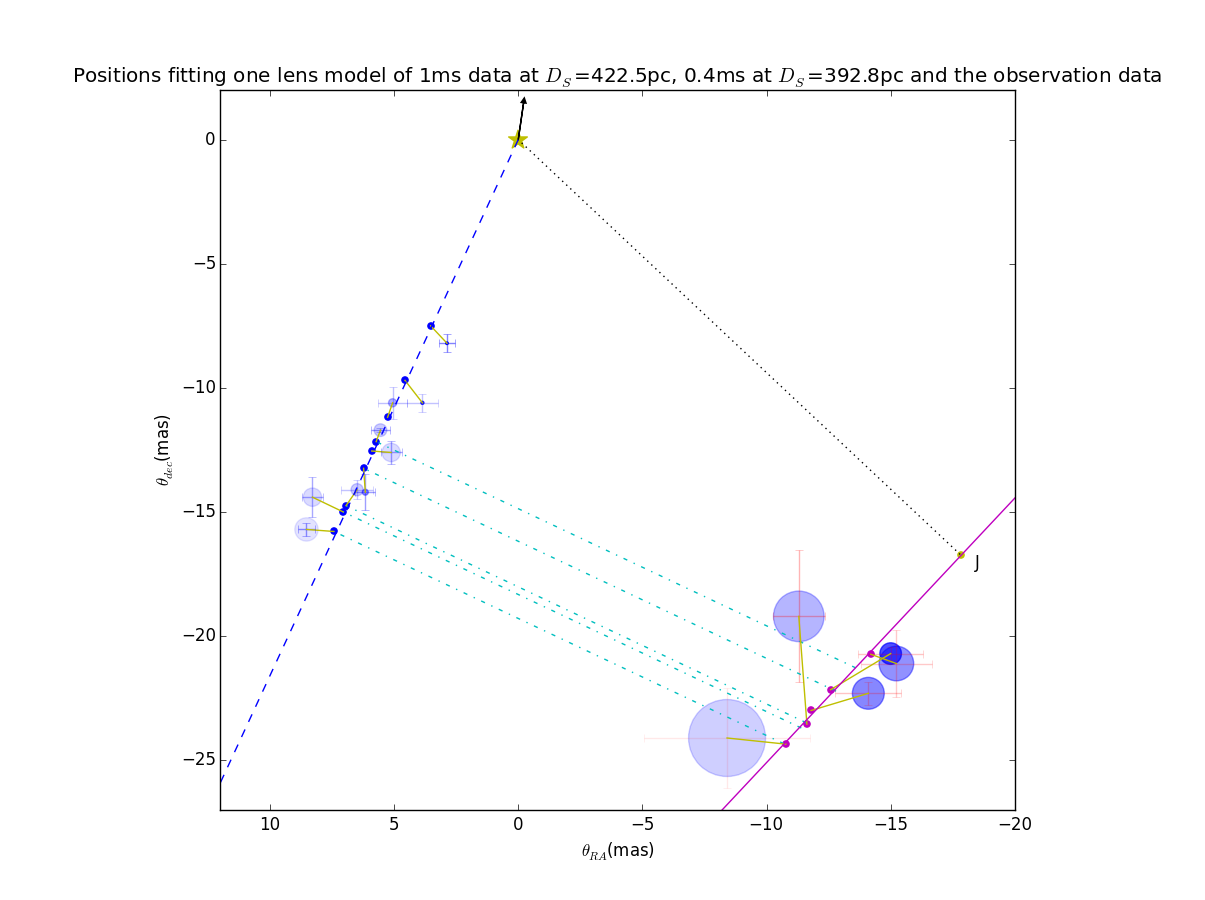
\includegraphics[width=0.8\textwidth, angle=0]{One_lens_640_392_422.png}
%\includegraphics{zN.eps}
%\caption{Same Observation data with the previous plot, this time we put the points with time delay lie in the range $1$ms at the screen that is $422.5$ pc away from us, which fitts better with the observation data. Velocity in this situation is $188499$m/s, with an angle $0.144147$ radian west of north. }
%\label{Onelens_392_422}
%\end{figure*}

\begin{figure}
\centering
%\epsscale{1.0}
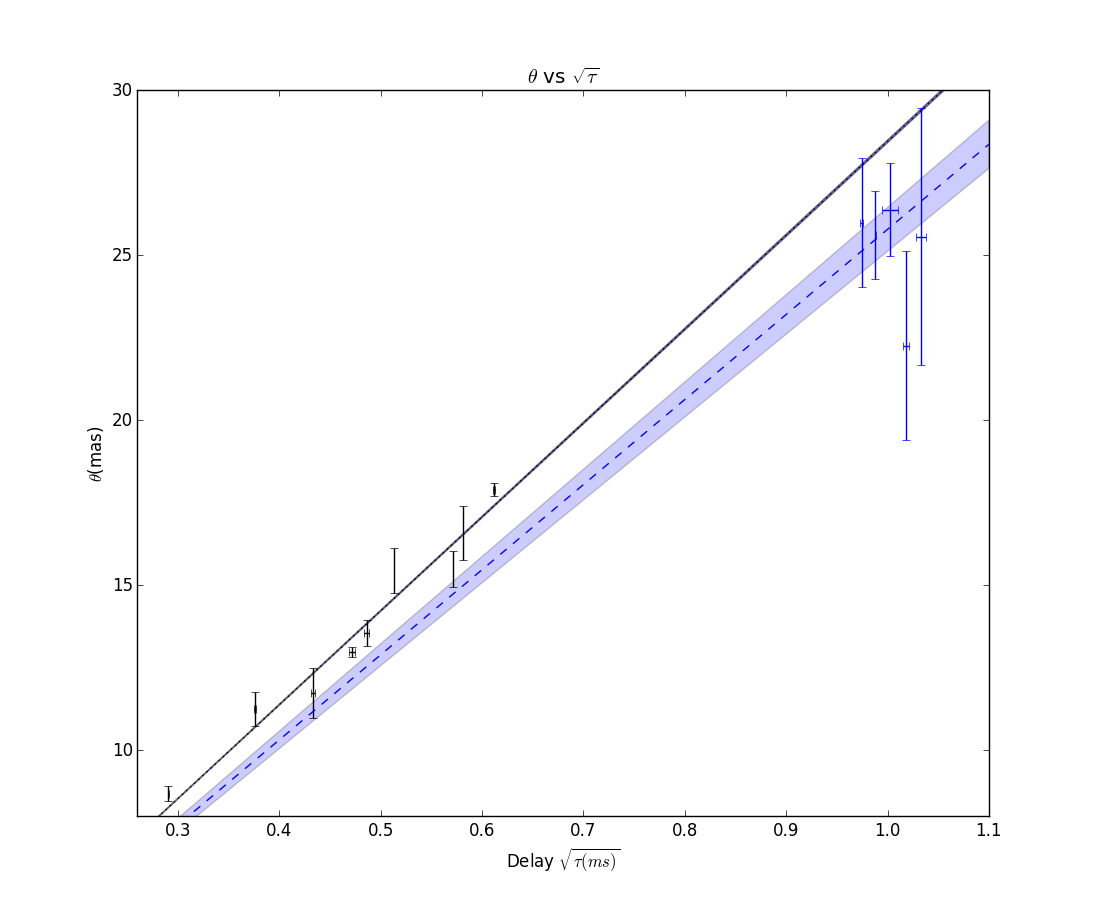
\includegraphics[width=1.0\linewidth, angle=0]{Theta_tau.png}
\caption{${\theta}$ vs ${\sqrt{\tau}}$. Two separate lines through the origin were fitted to the points sampled among the $0.4$ ms group and $1$ ms group. The solid line is the fitted line of the 0.4ms positions, where $k=28.51$ with an error region of $\sigma_k=0.04$. The dashed lines are the fitted lines of the 1ms position, where $k=25.78$ with an error region of $\sigma_k=0.66$.
}
\label{thetatau}
\end{figure}








%\begin{figure*}
%\centering
%\epsscale{1.0}
%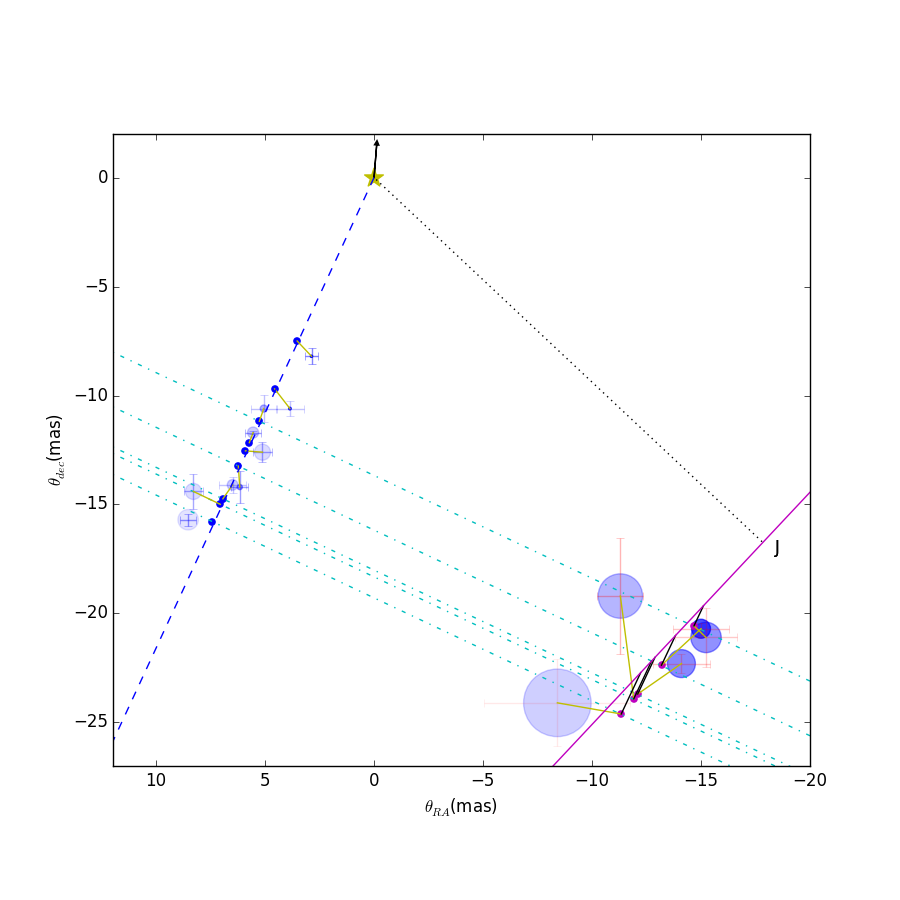
\includegraphics[width=1.0\textwidth, angle=0]{Double_lens_640_425_392.png}
%\caption{Fitted position of $1$ms and $0.4$ms data of double lens model and observation data.In both apexes regions, the position of the screen locate at $392.82$pc and $425$pc. Blue points on the left side are the points that fitted from the $f_D$ and $\tau$ of from the $0.4$ms observation. Blue line is the fitted line of $0.4$ms apex positions, with a $25.2$ degree west of the north. The points lie on the left side with errorbars, are the observation points together with their sample errors; while the transparent circles are plotted with population errors, where smaller transparent data are darker. Short solid lines between them are the matched positions of the apexes in $1ms$ region and $0.4ms$ region, which share the same $\theta_{\parallel}$. The points on the right side are the points that fitted from the $f_D$ and $\tau$ of the $1$ms observation with an avearage of four bandwidths. Solid line is the fitted line of these positions. Those points with errorbars nearby are the observation points together with their sample errors, while the transparent circles are plotted with population errors. The dotted line on the top right side is vertical to the solid line. Short solid lines connect the observation points and the fitted positions. Middle lines connect the $0.4$ms and $1$ms fitted positions with the same $\theta_{\parallel}$. The velocity of the pulsar is $191.4$km/s, with a degree $5.56$ degree west of north, is also marked out at the top of the figure.  }
%\label{Doublelens}
%\end{figure*}

\begin{figure*}
\centering
%\epsscale{1.0}
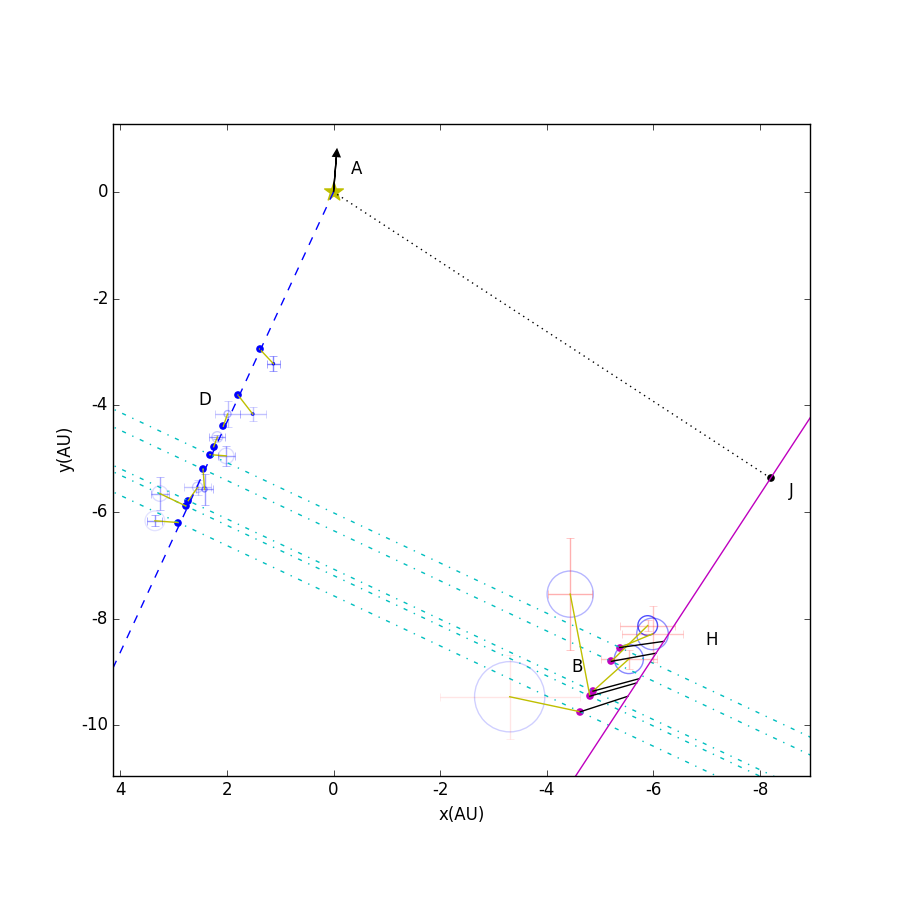
\includegraphics[width=1.0\textwidth, angle=0]{Double_lens_xy.png}
\caption{Observed and calculated angular positions of $0.4$ ms and $1$ ms data in double lens model. x axis and y axis are the relative distance to the position of the pulsar in Right Ascension direction and declination direction, on a 2D plane that is transverse to the line of sight. The position of the screen locate at $392.8$ pc and $425.0$ pc respectively. Scatter points on the left side, marked with letter D, are the calculated positions from the $0.4$ ms apexes observation. Dash line is the fitted line of $0.4$ ms apexes positions, with a angle $\gamma=-25.2\degree$  east of north. The points lie on the left side with errorbars, are the observation points with their sample errors; while the circles are plotted with population errors. Short solid lines between them are the matched positions of the observation positions and the calculated positions. The scatter points on the right side, marked with letter B, are the calculated lensed image on lens 1 from $1$ ms group. The short solid line connects the lensed image one lens 1(observable) and lensed image 2(unobservable), marked with letter H. Long solid line is the fitted line of these positions. Those points with errorbars nearby are the observation points with their sample errors, while the circles are plotted with population errors. The dotted line on the top right side is vertical to the solid line, and the pedal is called J. Short light solid lines connect the observation points and the calculated positions in $1$ ms group. Middle dot dash lines connect the $0.4$ ms and $1$ ms calculated positions with the same $\theta_{1\parallel}$, which are lens 1. The proper motion of the pulsar is $192.6$ km/s, with an angle $\epsilon=-4.59\degree$ east of north, is marked with an arrow from the star, point A the position of the pulsar, at the top of the figure.}
\label{Doublelens}
\end{figure*}


\begin{figure}
\centering
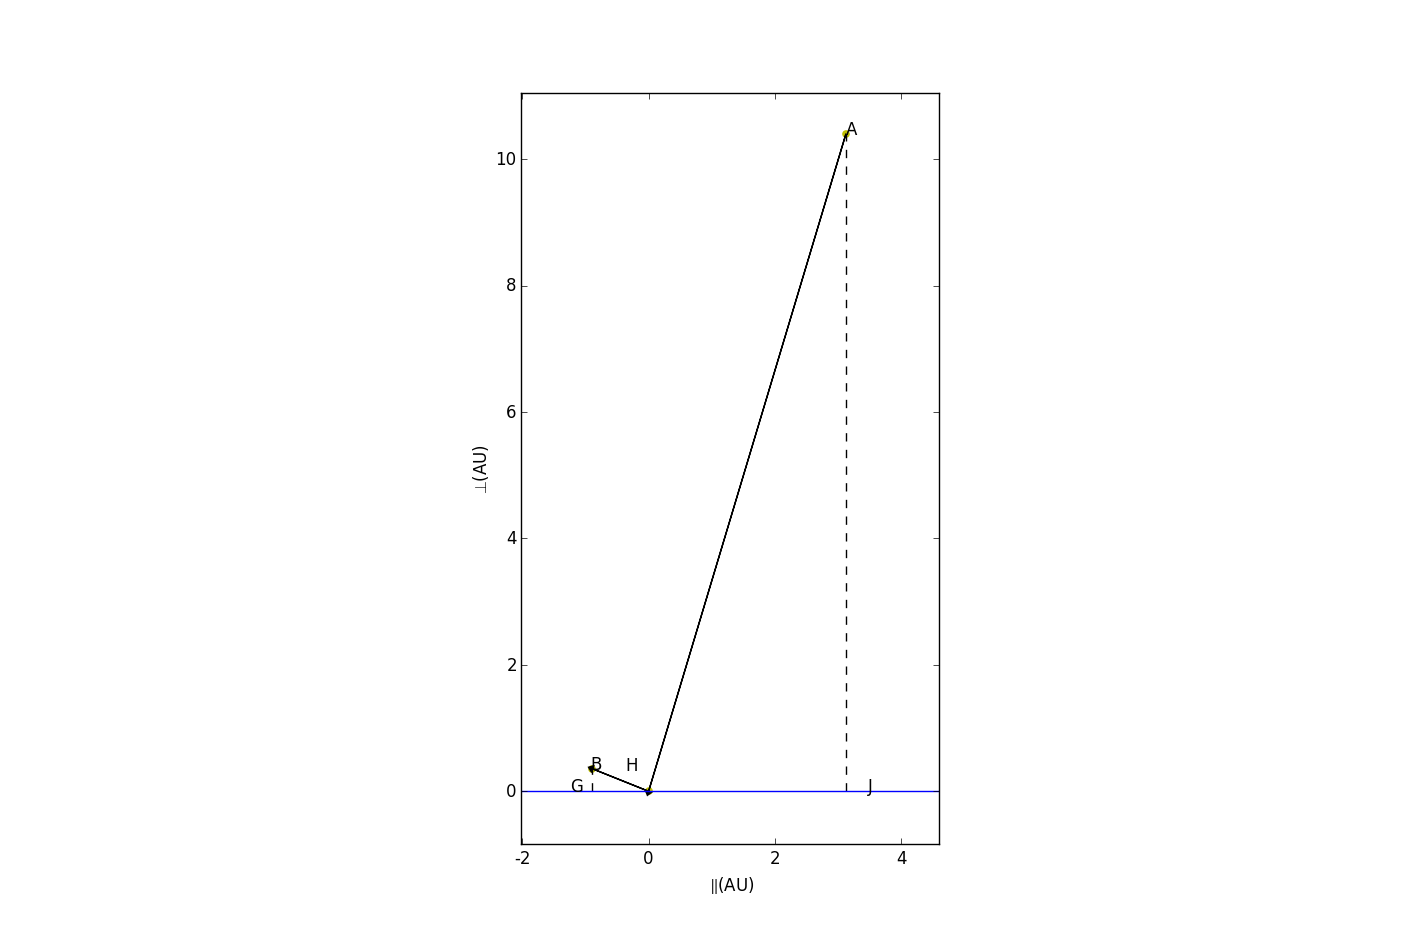
\includegraphics[width=1.0\linewidth,scale=1.0]{First_reflection.png}
\caption{Refraction on lens 2. 
%The x axis marks the distance in the direction that is parallel to lens 2, and the y axis marks the distance in the direction that is transverse to the lens 2. 
A is the position of the pulsar. H is the lensed image on lens 2. B is the lensed image on lens 1. J is the pedal of A to lens 2, and G is the pedal of B to lens 2. $v_{\rm JH}$ and $v_{\rm HG}$ should be equal, which is described in Section \ref{doublelensmodel}. In this case, $\theta_{1\parallel} =-17.44$ mas.}
\label{first_reflect}
\end{figure}

\begin{figure}
\centering
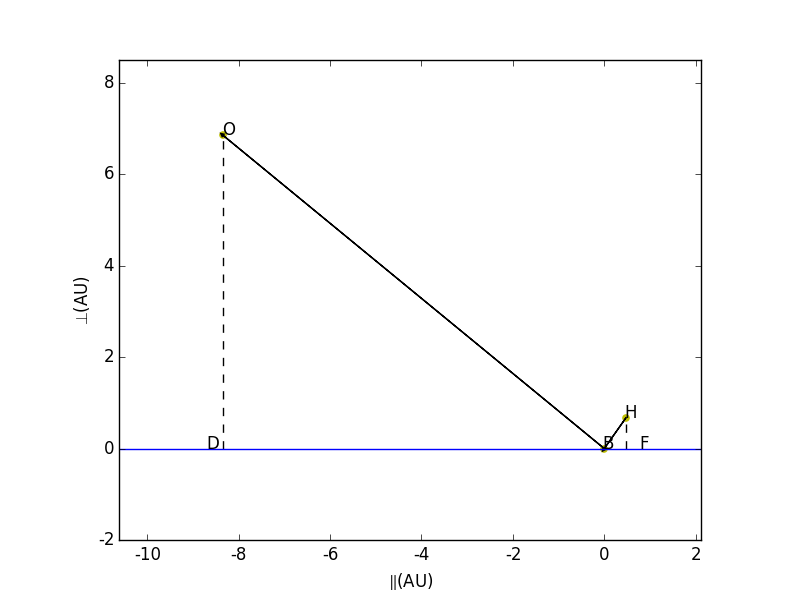
\includegraphics[width=1.0\linewidth]{Second_reflection.png}
\caption{Refraction on lens 1. 
%x axis marks the distance in the direction that is parallel to the second lens, and the y axis marks the distance in the direction that is transverse to the second lens. 
H is the lensed image on lens 2. B is the lensed image on lens 1. O is the position of the observer. F is the pedal of H to lens 2, and D is the pedal of O to lens 2. $v_{\rm FB}$ and $v_{\rm BD}$ should be equal, which is described in Section \ref{doublelensmodel}. In this case, $\theta_{1\parallel} = -17.44$ mas. }
\label{second_reflect}
\end{figure}

\begin{figure}
\centering
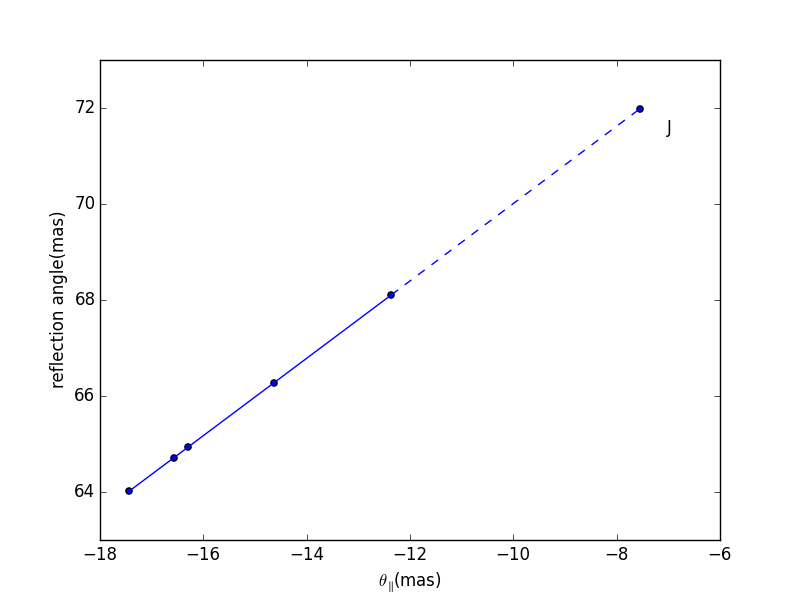
\includegraphics[width=1.0\linewidth]{Reflection_angle.png}
\caption{  ($\pi$-$\protect\angle$AHB) vs $\theta_{1\parallel}$.
%vs $\theta_{\parallel}$.}
$\beta_J$ is calculated with J as the lensed image on lens 2, and $\theta_{1\parallel}=-3.21$ mas.}
\label{vtrans}
\end{figure}



\section{Possible Improvements}

We discuss several strategies which can improve on the solution
accuracy.  The single biggest improvement would be to monitor over a
week, when the pulsar crosses each individual lens, including both
lensing systems.

Angular resolution can be improved using longer baselines, for example
adding a GMRT-GBT baseline doubles the resolution.  Observing at
multiple frequencies over a longer period allows for a more precise
measurement: when the pulsar is between two lenses, the refraction
angle $\beta$ is small, and one expects to see the lensing at higher
frequency, where the resolution is higher, and distances between
lenses positions can be measured to much higher accuracy.

Holographic techniques \citep{2008MNRAS.388.1214W,2014MNRAS.440L..36P}
may be able to measure delays, fringe rates, and VLBI positions
substantially more accurately.  Combining these techniques, the
interstellar lensing could conceivably achieve distance measurements
an order of magnitude better than the current published effective
distance errors.  This could bring most pulsar timing array targets
into the coherent timing regime, enabling arc minute localization of
gravitational wave sources, lifting any potential source confusion.

Ultimately, the precision of the lensing results would be limited by
the fidelity of the lensing model.  In the inclined sheet model, the
images move along fold caustics.  The straightness of these caustics
depends on the inclination angle, which in turn depends on the
amplitude of the surface waves.  

\section{Conclusions}

We have applied the \citep{2014MNRAS.442.3338P} inclined
sheet model to archival apex data of PSR B0834+06.  The data is well
fit by two linear lensing screens, with nearly plane-parallel
geometry.  This appears a natural consequence of very smooth
reconnection sheets, and are an unlikely outcome of ISM turbulence.
These results, if extrapolated to multi-epoch observations of binary
systems, this might result in accurate distance determinations.


\section{Acknowledgements}

We thank NSERC for support.


\newcommand{\araa}{ARA\&A}   % Annual Review of Astronomy and Astrophys.
\newcommand{\afz}{Afz}       % Astrofizica
\newcommand{\aj}{AJ}         % Astronomical Journal
\newcommand{\azh}{AZh}       % Astronomicekij Zhurnal
\newcommand{\aaa}{A\&A}      % Astronomy and Astrophysics
\newcommand{\aas}{A\&AS}     % Astronomy and Astrophys. Supplement Series
\newcommand{\aar}{A\&AR}     % Astronomy and Astrophysics Review
\newcommand{\apj}{ApJ}       % Astrophysical Journal
\newcommand{\apjs}{ApJS}     % Astrophysical Journal Supplement Series
\newcommand{\apjl}{ApJ}      % Astrophysical Journal Letters
\newcommand{\apss}{Ap\&SS}   % Astrophysics and Space Science
\newcommand{\baas}{BAAS}     % Bulletin of the American Astron. Society
\newcommand{\jaa}{JA\&A}     % Journal of Astronomy and Astrophysics
\newcommand{\mnras}{MNRAS}   % Monthly Notices of the Roy. Astron. Society
\newcommand{\nat}{Nat}       % Nature
\newcommand{\pasj}{PASJ}     % Publ. of the Astron. Society of Japan
\newcommand{\pasp}{PASP}     % Publ. of the Astron. Society of the Pacific
\newcommand{\paspc}{PASPC}   % Publ. Astron. Soc. Pacific Conf. Proc.
\newcommand{\qjras}{QJRAS}   % Quart. Journal of the Royal Astron. Society
\newcommand{\sci}{Sci}       % Science
\newcommand{\solphys}{Solar Physics}       % 
\newcommand{\sova}{SvA}      % Soviet Astronomy
\newcommand{\aap}{A\&A}
\newcommand\jcap{{J. Cosmology Astropart. Phys.}}%
\newcommand{\prd}{Phys. Rev. D}


\bibliography{distance}
\bibliographystyle{mn2e}


\label{lastpage}

\end{document}
